
%: ----------------------- physics file header -----------------------
\chapter{Overview of Relevant Physics}

% the code below specifies where the figures are stored
\ifpdf
    \graphicspath{{physics/figures/PNG/}{physics/figures/PDF/}{physics/figures/}}
\else
    \graphicspath{{physics/figures/EPS/}{physics/figures/}}
\fi

% ----------------------------------------------------------------------
% ----------------------- Physics content -------------------------
% ----------------------------------------------------------------------
\section{The Standard Model}
The standard model of particle physics is our current best way of understanding
all particle interactions that have so far been observed.
It's defining aspect is as a gauge theory in which all interactions
preserve a local $SU{(3)}_C \times SU{(2)}_L \times U{(1)}_Y$ symmetry, where
$C$, $L$, and $Y$ respectively indicate color, left-hand chirality and weak hyperchange.
These symmetry groups specify the number of bosons that mediate each...

The $SU({(3)}_C$ symmetry corresponds to the strong nuclear force and quark/gluon
interactions.

\section{Neutrinos}
Neutrinos were first hypothesized by Wolfgang Pauli in 1930.
The motivation for the proposal the apparent violation of energy
conservation in $\beta$ decay \citep{pauli_letter}.
Several years after Pauli's speculative proposal Enrico Fermi offered
a thorough model of beta decay that conserved energy using the neutrino
\citep{fermi_beta_decay}.
Fermi's model predicted such a small cross-section for the neutrino that some
doubted it would ever be observed \citep{bethe_impossible_to_observe}.
However, roughly two decades after its initial proposal, Frederick Reines \&
Clyde Cowan performed an experiment that involved bombarding a tank of cadmium
doped water with anti-neutrinos from nuclear reactor.
Doing this they were able to observe the rate and energy of inverse $\beta$
decays that occurred.
The results were consistent with Fermi's model of $\beta$ decay and were
considered a confirmation of the neutrino's existence.

\subsection{Neutrino Flavor}
The first experimental evidence for neutrino flavor came in 1962 from an
experiment \citep{lederman_muon_flavor} that studied the interactions of
neutrinos that came from muon decay, and the interactions of neutrinos
from beta decay.
The experiment observed that neutrinos from came from muon decay would produce
muons upon interacting in a detector.
And neutrinos produced from $\beta$ decay would create electrons in the
detector.
This lead to the conclusion that there are two different varieties of neutrino,
the $\nu_e$ and the $\nu_{\mu}$, and the idea that lepton flavor is conserved.
The third lepton generation, the $\tau$ and the $\nu_{\tau}$ was discovered 13
years later in 1975 \citep{tau_discovery}.
% It's worth noting that lepton flavor conservation was not predicted or required
% by the standard model, for that reason it's known as an 'accidental symmetry'.
% ^^^^Not true??? Lepton number is an accidental symmetry, idk about lepton
% flavor Also the definition of accidental symmetry has to do with term in the
% lagrangian being to high dimensional (according to wikipedia) not what I
% said....though they might be the same somehow

\subsection{Neutrino Interactions}
The neutrino interacts almost exclusively via the weak interaction.
In principle it also interacts gravitationally and it has a non-vanishing
magnetic moment so it can interact electromagnetically, but these
interaction potentials are so small they can be neglected in all practical
cases~\cite{neutrino_magmom}.
The weak interaction has a number of aspects that limit the sort of neutrino
interactions that can occur. The first aspect is lepton flavor conservation,
all weak interactions conserve both the total lepton number of a system, but also
the total lepton flavor of the system as well.
This leads to nearly all interactions involving a neutrino also involving the
same flavor charged lepton.
The second aspect is that the weak interaction is known to be chiral,
only left-handed particles and right-handed anti-particles interact weakly.
Since neutrinos only interact weakly, the only detectable varieties of neutrino
is the left-handed neutrino $\nu^{L}$  and the right-handed anti-neutrino $\overline{\nu}^{R}$.

Detailed here are the neutrino interactions that are relevant to this work, a more
complete overview of neutrino interactions is available in Ref~\cite{XXX}.
\subsubsection{Neutrino-Nuclear Interactions}
There are two varieties of neutrino nuclear interactions that are most
relevant for this work,
both are coherent
the charged current interaction with a neutron, and the
neutral current interaction with a proton or neutron.
\begin{figure}
        \centering
        \begin{feynman}
            \fermion[label=$e^{-}$]{0.00, 0.00}{1.00, 1.00}
            \fermion[label=$\nu_{e}$]{1.00, 1.00}{0.00, 2.00}
            \electroweak[label=$W^{+}$]{1.00, 1.00}{2.0, 1.00}
            \fermion[label=$\nu_{e}$, flip=true]{2.00, 1.00}{3.0, 0.00}
            \fermion[label=$e^{-}$, showArrow=true, flip=true]{2.0, 1.00}{3.00, 2.00}
        \end{feynman}
\end{figure}
\subsubsection{Neutrino-Electron Elastic Scattering}
\begin{figure}
    \begin{subfigure}[t]{0.53\textwidth}
        \centering
        \begin{feynman}
            \fermion[label=$e^{-}$]{0.00, 0.00}{1.00, 1.00}
            \fermion[label=$\nu_{e}$]{1.00, 1.00}{0.00, 2.00}
            \electroweak[label=$W^{+}$]{1.00, 1.00}{2.0, 1.00}
            \fermion[label=$\nu_{e}$, flip=true]{2.00, 1.00}{3.0, 0.00}
            \fermion[label=$e^{-}$, showArrow=true, flip=true]{2.0, 1.00}{3.00, 2.00}
        \end{feynman}
    \end{subfigure}
    \begin{subfigure}[t]{0.53\textwidth}
        \centering
        \begin{feynman}
            \fermion[label=$\nu_{x}$]{0.00, 0.00}{1.00, 1.00}
            \fermion[label=$\nu_{x}$]{1.00, 1.00}{0.00, 2.00}
            \electroweak[label=$Z$]{1.00, 1.00}{2.0, 1.00}
            \fermion[label=$e^{-}$, flip=true]{2.00, 1.00}{3.0, 0.00}
            \fermion[label=$e^{-}$, showArrow=true, flip=true]{2.0, 1.00}{3.00, 2.00}
        \end{feynman}
    \end{subfigure}
    \label{fig:feynman_es}
\end{figure}

Neutrino-electron elastic scattering (ES) is an important neutrino interaction
channel, for this work it is the main interaction through which neutrinos are
detected.
The ES process is $\nu_{\mathrm{x}} + e^{-} \rightarrow \nu_{mathrm{x}} +e^{-}$.
A similar process exists for anti-neutrinos, but the focus here is on the
neutrino ES interaction.

Figure~\ref{fig:feynman_es} shows the tree level feynman diagrams for the charged
current (CC) elastic scattering interaction~\ref{fig:feynman_es_cc} and the
neutral current (NC) elastic scattering interaction~\ref{fig:feynman_es_nc}.
The neutral current interaction is shown to involve $\nu_{\mathrm{x}}$ where $x=\mathrm{e, \mu, \tau}$,
and the charged current interaction involves only $\nu_{\mathrm{e}}$.
The charged current interaction is available to neutrinos of all flavors,
however, for a few reasons only the electron flavor version of the interaction
is available for solar neutrinos.

The intial electron on the left hand side of the interaction is usually understood to
be from an atom within target the detector, and therefore at rest within
the lab frame.
So the total energy in the interaction is simply $E = E_{\nu} + m_{e}$.
For even the highest energy solar neutrinos $E<20$\,MeV, far less that muon
rest mass of $m_{\mu}=105.7$\,MeV/$\text{c}^{2}$ or tau mass $m_\tau = 1776.8$\,MeV/$\text{c}^{2}$.
Meaning a muon or tau cannot be created; the electron with a rest mass
of $m_{e}=0.511$\,MeV/$\text{c}^{2}$ is the only charged lepton that can
be created from the CC-ES interaction for solar neutrinos.
And since lepton flavor is conserved in weak interactions, the electron neutrino
is the only neutrino that can produce an electron, therefore the electron
neutrino is the only neutrino flavor that can undergo the charged-current
elastic scattering interaction.

%TODO need citations here
In practice this means that the cross section for the elastic scattering process
is larger for $\nu_{e}$ than it is for a $\nu_\mu$ or $\nu_\tau$,
and the cross-section for a $\nu_\mu$ is the same as that for a $\nu_\tau$.
The differential cross section of for the diagrams shown in Fig~\ref{fig:feynman_es}
can be calculated as
\begin{equation}
    \frac{d\sigma}{dT_{\mathrm{e}}}\left(E_{\nu}\text{, }T_{\mathrm{e}}\right)=
    \frac{\sigma_{0}}{m_{\mathrm{e}}}\left[g_{1}^{2} + g_{2}^{2}\left(1 - \frac{T_{\mathrm{e}}}{E_{\nu}}\right)^{2} -g_{1}g_{2}\frac{m_{\mathrm{e}}T_{\mathrm{e}}}{E_{\nu}^{2}}\right]\text{,}
\end{equation}
where,
\begin{equation}
    \sigma_{0} = \frac{2G^{2}_{\mathrm{F}}m_{\mathrm{e}}^{2}}{\pi}\text{.}
\end{equation}
For $\nu_{x} = \nu_{e}$
\begin{equation}
    g_{1} = \frac{1}{2} + \sin^{2}\theta_{\mathrm{W}}\text{,}
\end{equation}
and
\begin{equation}
    g_{2} = \sin^{2}\theta_{\mathrm{W}}\text{.}
\end{equation}

For $\nu_{x} = \nu_{\mu}$ or $\nu_{x} = \nu_{\tau}$ $g_{1}$ and $g_{2}$ is
given by,
\begin{equation}
    g_{1} = \sin^{2}\theta_{\mathrm{W}} - \frac{1}{2}\text{,}
\end{equation}
and
\begin{equation}
    g_{2} = \sin^{2}\theta_{\mathrm{W}}\text{.}
\end{equation}

Since the electron scattering is elastic the kinematics of the interaction
leave only free parameter, the outgoing electron direction, with respect
to the incoming neutrino direction, $\theta$.
For a recoil electron with a given value for $\theta$ the electron kinetic energy is
given by
\begin{equation}
    T_{\mathrm{e}}=\frac{2m_{\mathrm{e}}E_{\nu}^{2}\cos^{2}\theta}{(m_{\mathrm{e}}+E_{\nu})^2 - E_{\nu}^{2}\cos^2\theta}\text{.}
    \label{eqn:es_te_theta}
\end{equation}
This relationship can be used to produce the differential cross-section
\begin{multline}
    \frac{d\sigma}{d\cos\theta}=\sigma_{0}\frac{4E_{\nu}^{2}(m_{\mathrm{e}}+E_{\nu}^{2})^2\cos\theta}{\left[(m_{\mathrm{e}}+E_{\nu}^{2} -E_{\nu}^{2}\cos^2\theta)\right]^2}\\
    \left[g_{1}^{2} + g_{2}^{2}\left(1 - \frac{2m_{\mathrm{e}E_{\nu}\cos^{2}\theta}}{(m_{\mathrm{e}}+E_{\nu})^2 -E_{\nu}^{2}\cos^2\theta} \right)^{2} - g_{1}g_{2}\frac{2m_{\mathrm{e}^{2}}\cos^{2}\theta}{(m_{\mathrm{e}}+E_{\nu})^{2}-E_{\nu}^{2}\cos^{2}\theta}\right]
    \text{.}
\end{multline}
And finally the maximum energy a recoil electron will have can be found by
setting $\cos\theta=1$ in equation~\eqref{eqn:es_te_theta}, this yields
\begin{equation}
    T_{e}^{\max}(E_\nu) = \frac{2E_{\nu}^{2}}{m_{\mathrm{e}}+ 2E_{\nu}^{2} }\text{.}
\end{equation}

Figure~\ref{XXX} shows the differential cross-sections for a 10\,MeV neutrino.
The fact that the scattering cross-section is so peaked in $\frac{d\sigma}{d\cos\theta}$
is very useufl for neutrino experiments because it means the electron direction
is almost always nearly co-linear with the neutrino direction.
Unforunately, since the cross-section is nearly flat in $T_{\mathrm{e}}$
the electron energy conveys almost no information about the incoming neutrino
energy.
The kinematics and cross-section of the out-going neutrino is also
well predicted with respect to $\cos\theta$, however the out-going
neutrino is of little interest because it in general cannot be detected.

%TODO look at PDG review and discuss uncertainties.

\subsection{Neutrino Oscillations}
\label{sec:neut_osc}
Neutrino oscillation is a result of the fact that neutrino flavors do not have
well defined masses, instead neutrino flavor states are quantum superposition
And conversely, mass states can be described as a superposition of flavor states.
This can be stated more precisely as
\begin{equation}
    \ket{\nu_{i}} = U_{i\ell}\ket{\nu_\ell}
\end{equation}
Where $\ket{\nu_\ell}$ represents the neutrino flavor states, $\ket{\nu_i}$
represents the mass states, and $U_{i\ell}$ describes the mixing of these
states. $U$ is known as the Pontecorvo-Maki-Nakagawa-Sakata (PMNS) matrix,
and it is exactly analogous to the Cabibbo-Kobayashi-Maskawa (CKM) matrix used
to describe quark mixing.
In the simplest case where the weak states and the mass states are the same
$U$ would just be the identity matrix;
Under the assumption that there are three flavor states and three mass states
$U_{i\ell}$ must be unitary so that the probability of observing
a neutrino in any state is 1.
It is known from observations of Z boson decay products that
there are only three ``active'' neutrino flavors~\cite{Zbosondecaypaper}.
Where active here means that the neutrino participates in
weak interactions.

It is typical to characterize $U$ with three angles
($\theta_{12}$, $\theta_{13}$, $theta_{23}$) and a complex
phase $\delta_{cp}$. Doing so allows for the SU(3) matrix to
be decomposed into two SO(2) matrices and one SU(2) matrix,
$$U_{12} =
\begin{bmatrix}
    \cos\theta_{12} & \sin\theta_{12} & 0  \\
    -\sin\theta_{12}& \cos\theta_{12} & 0  \\
    0 & 0 & 0  \\
\end{bmatrix},
$$
$$
U_{13} =
\begin{bmatrix}
    \cos\theta_{13} & 0 & \sin\theta_{13}e^{-i\delta_{cp}}\\
    0 & 0 & 0  \\
    -\sin\theta_{13} e^{-i\delta_{cp}} & 0 & \cos\theta_{13}  \\
\end{bmatrix},
$$
$$
U_{23} =
\begin{bmatrix}
    0 & 0 & 0  \\
    0 & \cos\theta_{23} & \sin\theta_{23} \\
    0 & -\sin\theta_{23} & \cos\theta_{23}   \\
\end{bmatrix}.
$$
These matrices can be multiplied to produce the full mixing matrix
$U = U_{23}U_{13}U_{12}$

The mixed nature of neutrino flavor and mass states gives rise to oscillations
in the flavor content of propagating neutrinos.
By definition the neutrino mass states are eigenstates of the vacuum Hamiltonian
\begin{equation}
    H\ket{\nu_{i}} = E_{i}\ket{\nu_{i}}\text{,}
\end{equation}
where the energy is given by the standard relativistic energy equation,
\begin{equation}
    E_{i} = \sqrt{{(p_{i}c)}^{2} + {(m_{i}c^{2})}^2}\text{.}
\end{equation}
It is typical to make the assumption that all neutrino mass states have the same
momentum, $p_{i} = p$, and this is the assumption I'll user here as well.
The equal momentum assumption allows for a straightforward derivation of the
correct description of neutrino oscillations, but it is not well motivated.
A thorough discussion of the assumption is available in Ref~\cite{Ahkmedov_Quantum}.

Applying Schrodinger's equation,
\begin{equation}
    i\frac{d}{dt}\ket{\nu_{i}(t)} = H\ket{\nu_{i}(t)} = E_{i}\ket{\nu_{i}(t)}\text{,}
\end{equation}
results in,
\begin{equation}
    \ket{\nu_{i}(t)} = e^{-iE_{i}t}\ket{\nu_{i}(t=0)}\text{.}
    \label{eqn:mass_state_tevol}
\end{equation}

This time evolution of mass eigenstates can be used to then describe the state
of a neutrino that is created in a electron flavor eigenstate.
\begin{equation}
\ket{\nu(t=0)} = \ket{\nu_{e}} = U_{1e}\ket{\nu_1} + U_{2e}\ket{\nu_{2}} + U_{3e}\ket{\nu_{3}}
    =\sum_{i=1}^{3}U_{ie}\ket{\nu_{i}}
\end{equation}

Each of the mass states' time evolution can be immediately written down from
Equation~\eqref{eqn:mass_state_tevol},
\begin{equation}
    \ket{\nu(t)} = \sum_{i=0}^{3} U_{ie}e^{-iE_{i}t}\ket{\nu_{i}}\text{.}
    \label{eqn:e_state}
\end{equation}

From Eq.~\eqref{eqn:e_state} the quantity that's often of the most interest
is the survival probability, defined as
\begin{equation}
    P_{ee}(t) = \abs{\braket{\nu_{e}}{\nu(t)}}^{2}\text{.}
\end{equation}
$P_{ee}(t)$ can be understood as the probability that a neutrino, produce in
an electron flavor state, will be detected as an electron flavor state a time
$t$ later.
The survival probability for the state given in~\eqref{eqn:e_state} is
\begin{equation}
    P_{ee}(t) = \sum_{i,j}\abs{U_{ei}}^2\abs{U_{ej}}^2e^{-i(E_{i} - E_{j})t}\text{.}
\end{equation}
It is useful to separate out the terms where $i=j$,
\begin{equation}
    P_{ee}(t) = \sum_{i}\abs{U_{ei}}^4 + \sum_{i,j\text{, }j \ne i}
    \abs{U_{ei}}^2\abs{U_{ej}}^2e^{-i(E_{i} - E_{j})t}\text{.}
\end{equation}
Here we can see there are terms that oscillate with time, and terms that do
not.

A few more simplifications are commonly done, using the equal momentum
assumption mentioned earlier and the fact the neutrino rest mass is
very small, the energy differences can be simplified,
\begin{equation}
    E_{i} - E_{j} = \sqrt{p^{2} + m_{i}^{2}} - \sqrt{p^{2} + m_{j}^{2}} \approx
    p^{2} - p^{2} + \frac{m_{i}^2}{2p} - \frac{m_{j}^2}{2p}\text{.}
\end{equation}
To good approximation $p=E$, so
\begin{equation}
    E_{i} - E_{j} = \frac{\Delta m^{2}_{ij}}{2E}\text{,}
\end{equation}
where the definition of the mass-squared splittings is used,
\begin{equation}
    \Delta m^{2}_{ij} = m^{2}_{i} - m^{2}_{j}\text{.}
\end{equation}

The final simplification is to assume that the neutrino is moving very close
to the speed of light, therefore any flavor oscillations over time will also
occur at a distance $L$ from the neutrino's creation.
All this gives
\begin{equation}
    \label{eqn:pee_adiabatic}
    P_{ee}(L,E) = \sum_{i}^{3}\abs{U_{ei}}^4 +
    \sum_{i,j\text{, }j \ne i}^{3}
    \abs{U_{ei}}^2\abs{U_{ej}}^2e^{-i\left(\frac{\Delta m^{2}_{ij}}{2E}L\right)}\text{.}
\end{equation}

Figure XXX shows this survival probability with mixing parameters matching those
given in~\cite{PDG2016}.


\subsubsection{Matter Enhanced Oscillations}
When neutrino propagate through matter this oscillation is altered.
The local density of other particles modifies the vacuum Hamiltonian,
adding a weak interaction potential.
This interaction comes from a neutral current interaction of the form
shown in $TODO$, or a flavor dependent charge current interaction with the
leptons around the neutrino.
Since nearly all matter contains a much higher density of electrons
than the other flavors of charged lepton, the charged current reaction
modifies the electron neutrino potential and not the potential for the muon
or tau neutrion.
The result is that the electron density through which a neutrino propagates
can modify the effective mass-splitting and mixing angle for the electron
neutrino.
For a given neutrino energy $E_{\nu}$ there exists an electron density for which
the effective mixing angle is maximal, this is known as the resonant density.

The masses of the neutrino mass states are not known, there are limits placed
on the sum of the neutrino masses from observations of tritium decay, and
from astronomical considerations. % TODO add citation.


\begin{equation}
    H \ket{\nu_i} = m_i \ket{\nu_i}
\end{equation}

\subsection{Adabaticity}
The adabiticity of neutrino oscillation refers if mass state composition
of a neutrino state changes or not, if it does change then the neutrinos
oscillation is non-adiabatic.
A specific example is if you imagine a neutrino state that's a pure vacuum mass-1
state,
\begin{equation*}
    \ket{\Psi_{\nu}} = \ket{\nu_{1}}
\end{equation*}
suddenly enters a region of significant matter density where the mass states
are now $\ket{\nu_{k}^\prime}$.
The neutrino state does not have time to evolve at all so the state
does not change, but it is not longer a pure eigenstate of the mixing
hamiltonian,
\begin{equation*}
    \ket{\Psi_{\nu}} = \ket{\nu_{1}} = \sum_{k=1}^{3} \braket{\nu_{k}^\prime}{\nu_{1}}\ket{\nu_{k}^\prime}\text{.}
\end{equation*}
Since the neutrino is no longer in a pure eigenstate the state will
now oscilate.

In contrast if the neutrino slowly enters the region of significant matter
density more slowly, then the neutrino state will smoothly evolve with the
eigenstate, $\ket{\nu_{1}} \rightarrow \ket{\nu_{1}^{\prime}}$.
And so the final state of the neutrino in the adiabatic case will be,
\begin{equation*}
    \ket{\Psi_{\nu}} = \ket{\nu_{1}^{\prime}}\text{.}
\end{equation*}

The adiabaticity of neutrino evolution will be discussed further in
Chapter~\ref{XXXChapChamleons}.

\subsection{Solar Neutrinos}
Nuclear reactions in the core of the sun provide energy to maintain a equilibrium
between gravitational forces and XXX forces.
There exists two seperate chains of nuclear reactions that are present in typical
stellar conditions, the $pp$-chain and the CNO-cycle. Figure XXX shows these
two reaction chains.
For the Sun the $pp$ chain
provides 99\% of the generated nuclear energy, and the CNO-cycle provides the remaining
1\%. For stars significantly more massive than the Sun, the CNO-cycle is the
main energy generating mechanism.

Within the $pp$-chain there are five process that produce neutrinos.
Since the Q-value the processes in the $pp$ chain are all well below the rest mass
of a muon or tau, the only charged lepton generated is electrons. And so from
lepton flavor conservation only electron flavor neutrinos are generated.
These neutrinos are produced with an energy spectrum shown in Fig. XXX.

The $hep$ and $\ce{^{8}B}$ reactions produce neutrinos with the highest
energies. Since the $hep$ reaction branching ratio is so low the flux
of $hep$ neutrinos is also very low compared to that of $\ce{^{8}B}$ neutrinos;
the $hep$ flux is expected to be XXX\% of the $\ce{^{8}B}$ flux.
So for water-Cherenkov detectors that have a typical threshold of a few MeV, $\ce{^{8}B}$ neutrinos
are the primary source of detectable solar neutrinos.

The uncertainty on the predicted $\ce{^{8}B}$ flux is relatively large, this comes mostly
from the uncertainty on the cross-sections and how those cross-sections change with
temperature, and uncertainties on the temperature profile within the core of the sun.
And since the $\ce{^{8}B}$ reaction has five preceding reactions the uncertainty on
 those reactions are part of the uncertainty on the $\ce{^{8}B}$ flux.

The uncertainty on the $pp$ and $pep$ neutrinos is much lower for two reasons. First, because
they are at early stage of the reaction chain, so their reaction rate is not dependent on any
other preceding interaction. The $pp$ reaction is also the main energy generating mechanism
for the Sun, so measurements of the total solar luminosity provide strict constraints on the
$pp$ flux as well.

Neutrinos created in the solar core can experience significant mixing effects from local
electron density.
One of the most interesting aspects to neutrino mixing within the Sun is the MSW-effect,
at a specific electron density a resonance occurs and neutrinos are maximally mixed.
The condition for an MSW-resonance between any two matter states is given by
\begin{equation}
    N_{e} = \frac{\Delta m^{2} \cos2\theta}{2\sqrt{2}EG_{F}}\text{.}
\end{equation}
This condition is met for a 10\,MeV at a solar radius of XXX, for the mixing parameters
given in XXX %cite pdg probably.
For neutrinos below XXX\,MeV this condition is not met at any point within the sun,
and so those neutrinos do not experience the MSW resonance.
Once a neutrino created in the core of the sun has travelled past a solar radius of $\approx$XXX
the solar electron density has dropped far enough that matter effects are no longer significant
and neutrinos are effectively travelling through vacuum. Once in the vacuum mixing dominated region

The effect neutrino mixing has on the neutrino flux is typically summarized by the
$\ce{^{8}B}$ survival probability, $P_{ee}(E_{\nu})$ over the energy range 0-15\,MeV,
shown in Fig~\ref{XXX}.

For solar neutrinos it's generally assumed that the neutrino states
will evolve adiabtically.
However, when the neutrino transitions through the MSW-resonance
the flavor composition of the mass states changes very rapidly,
so it's thought that this could lead to a non-adiabatic transition
between the mass-1 and mass-2 state~\cite{FIND CITATION}.
For solar neutrinos the effect this transition would have on the
neutrino survival probability is characterized with $P_{jump}$,
\begin{equation}
    P_{jump} = XXXX
\end{equation}
Experimental observations of solar neutrinos so far cannot distinguish if the
neutrino oscillation is fully adiabatic or not~\cite{GDOG Everything Under the sun???XXX}.




\subsection{Neutrino Experiments}
There's a long a diverse list of neutrino experiments that have contriubted to
our current understanding of neutrinos and neutrino oscillations.
I won't attempt to list them all here, but rather highlight the most immediatly
relevant to this work. A more compresive review can be found in \citep{FINDAREVIEW}.

\subsubsection{Homestake}
The first experiment to succesfully detect solar neutrinos was the Homestake
experiment.
The detector was composed of approximately 100000 gallons of dry cleaning fluid.
The choice of target was motivated by the high chlorine content in the cleaning
fluid. Neutrinos above an energy of XXX would interact with the chlorine via
beta decay, creating XXX. XXX would then decay to XXX with a half life of XXX.
Periodically $\ce{^{3}He}$ was bubbled through the
target liquid to extract the atoms of XXX that had been created. Once
extracted those atoms were observed with proportional counters to count the
number of XXX to XXX decays. The number of observed counts was proportional
to the solar neutrino interaction rate, and therefore the solar neutrino flux.

The homestake experiment ran from 1970 - 1990. %(XXX? is that right??)
The experiment was able to provide the first measurement of the solar neutrino
flux above XXX MeV. In 19XX they first reported a measure flux of
XXX, nearly a third of the expted rate which was XXX.
This deficiency became known as the solar neutrino problem, and it
was the first evidence for neutrino oscillation.
The deficiency was present across the entire lifetime of the Homestake experiment,
their final report flux was XXX.

\subsubsection{SNO}
\label{sec:sno}
The Sudbury Neutrino Observatory (SNO) is a water-Cherenkov detector located
roughly $2$\,km underground near Sudbury Ontario in Canada, it ran from
$1999$ to $2006$.
SNO was primarily a solar neutrino detector, it had the unique benefit of
being able to detect neutrinos through three different interaction channels,
each channel had it's own sensitivity to different flavor neutrinos.
This allowed for a measurment of the $^8B$ solar neutrino flux that was not
dependent on the flavor composition of the incoming neutrinos.
This was accoplished by using a heavy-water ($\ce{^{2}H_{2}O}$) target.
Heavy-water's primary neutrino interactions are the
electron scattering interaction (ES), a charged current nuclear reaction (CC),
and a neutral current nuclear reaction (NC).
%TODO add feynman diagrams for those reactions.
There exists both charged current and a neutral current versions of the
ES interaction; since electron neutrinos can interact through either
of the two where as muon or tau neutrinos can only elastic scatter throug the
neutral current version, the ES cross-section for electron neutrinos is larger
than the cross-section for muon and tau neutrinos.
The difference in cross-section is energy dependent, but it's roughly a factor
of 6 for solar neutrino energies. The neutral current and charged current ES reactions
are not treated seperately because there is no detectable signature that
would allow you to discrimate between the two.

The NC interaction on a deuteron can break apart the neutron and proton
that comprises the nucleus. $\nu_{e} + D -> p + n + \nu_{e}$.
The free-neutron can then capture on the deuterium forming tritium ($\ce{^{3}H}$)
and emitting an $XXX$\,MeV gamma. %TODO how often does it capture on oxygen?????
The NC reaction has no neutrino flavor preference, so a measure of the rate
of NC rate along with the process' cross-section provides a flavor independent
measurement of the solar neutrino flux.

The charged current interaction on a deuteron converts a neutron to a
proton and produces an electron.$\nu_{e} + D -> H + H + e^{-}$.
This reaction can only occur when the charged lepton and the neutrino are the same
flavor. So for typical matter this reaction only occurs for the electron flavor
neutrinos, and so it provides a measurement of the electron flavor content
of the solar neutrino flux.

SNO was able to seperate and count the events of each type of interaction,
providing them three independent measurements of solar neutrinos. And
the rates of each measurement had a different dependence on the flavor content
of solar neutrinos.


\subsubsection{Super Kamiokande}
Super Kamiokande (SuperK) is a 50\,kton cylindrical water cherekov detector.
It started running in $1996$ and has since made the most precise measurements of
atmospheric neutrinos and solar neutrinos so far.
It's the successor to the previous Kamiokande experiment, which was a significantly
smaller and had a higher energy threshold for detection.
SuperK can detect $\ce{^{8}B}$ solar neutrinos through only neutrino-electron elastic scattering,
they do not use a $\ce{D_{2}O}$ target and so are not sensitive to the
nuclear interactions that SNO used.
Their extremely large detector volume though provides them with far more exposure
than SNO could attain though. This results in a very precise measurement of the
elastic scattering rate.

The SuperK experiment seperates their dataset into 4 subsets, called
SuperK-I, SuperK-II, \textit{etc}. %TODO Roman numerals.
Each dataset covers several years of data taking.

\subsubsection{Borexino}
Borexino is 300\,ton spherical liquid scintillator detector~\cite{borexino_tdr}. Their detector
apparatus is similar to that of a water-Cherenkov detector, the significant difference
is that the water is replaced with pseudo-cumine, a liquid scintillator.
A charged particle moving through scintillator generates roughly 50-100 times
more light than a similar particle moving through just water.
Water-Cherenkov detector are typically limited in energy threshold
and energy resolution by the number of photons produced and detected, a liquid scintillator
detector solves this problem.  Scintillation light, unlike Cherenkov light,
is isotropic and provides no information about the direction the particle
was moving in.
\begin{figure}[htbp]
    \centering
    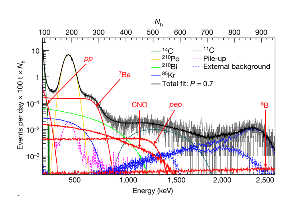
\includegraphics[width=1\textwidth]{borexino_spectrum}
    \caption[Borexino Spectrum] {}
\label{fig:borexino_spectrum}
\end{figure}

Water-Cherenkov detector are able to measure solar neutrinos by correlating the
direction of detected events with the position of the sun. Since Borexino is not
able to determine the direction of events within their detector, they instead
perform a spectroscopic measurement. The measurement requires
all sources of backgrounds to be accounted for and constrained from \textit{ex-situ}
measurements. Figure \ref{fig:borexino_spectrum} shows the observed spectrum by Borexino and the
spectrums of the constituent solar fluxes and backgrounds.

Borexino took data from 2007 to 2016, with a pause in 2010 to remove source
of radioactive backgrounds and improve the radio-purity of their detector.
With that data they've produced measurements of neutrino fluxes from the $\ce{^{7}Be}$,
$\ce{pep}$, $\ce{pp}$, and $\ce{^{8}B}$; they've also placed upper limits on the flux
of neutrinos from the CNO cycle and from the $hep$ solar reaction.
They're currently the only experiment to have measured the $\ce{pp}$ and $\ce{pep}$ neutrino
fluxes.

$XXX$ FIND TABLE\\
show spectrum and table of results

\subsubsection{KamLAND}
The Kamioka Liquid Scintillator Antineutrino Detector (KamLAND) is a liquid-scintillator experiment similar to Borexino.
It's primary physics goals were the detection of reactor anti-neutrinos via
inverse beta-decay (IBD),
but the experiment is also sensitive to solar neutrinos.
Performing a fit to the observed energy spectrum they were able to measure
the flux of $\ce{^{7}Be}$~\cite{kamland_be7} and $\ce{^{8}B}$~\cite{kamland_b8}.
The $\ce{^{8}B}$ flux is reported as the ``elastic-scattering'' flux $\Phi_{ES}$, the flux of
pure electron flavor neutrinos that would produce the observed event rate.
They, measure $\Phi_{ES\mathrm{,}\ce{^{8}B}} = 2.77 \pm 0.26(\mathrm{stat.}) \pm 0.32(\mathrm{syst.}) \times 10^6 \mathrm{cm}^{-2}\mathrm{s}^{-1}$

\begin{figure}[htbp]
\centering
\begin{subfigure}[b]{0.48\textwidth}
\centering
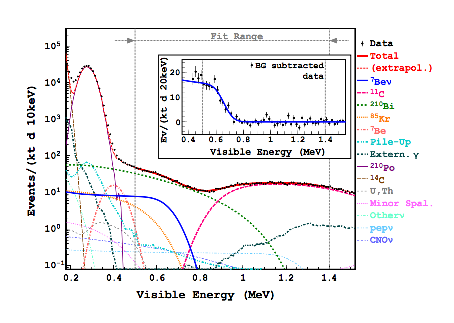
\includegraphics[width=\textwidth]{kamland_be7_spectrum}
\caption{}
\label{fig:kamland_be7}
\end{subfigure}
%\hfill
\begin{subfigure}[b]{0.48\textwidth}
\centering
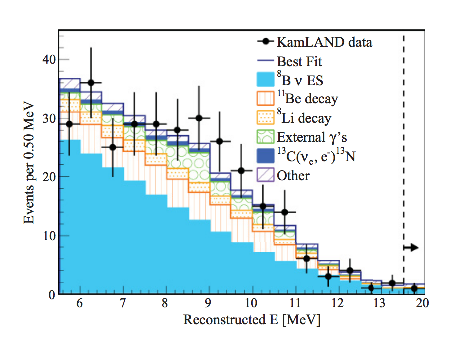
\includegraphics[width=\textwidth]{kamland_b8_spectrum}
\caption{}
\label{fig:kamland_b8}
\end{subfigure}
\caption{The observed reconstructed event energy spectrum for the Kamland Be7 flux measurement (a)
  and the 8B flux measurement (b). Figures from~\cite{kamland_be7} and~\cite{kamland_b8}.}
\label{fig:kamland_spectrum}
\end{figure}

Interestingly, KamLAND's reactor neutrino measurements~\cite{kamland_reactor} are
more relevant to the study of solar neutrinos than their solar neutrino measurements.
The long baseline (\urltilde180\,km) and low energy (\urltidle3\,MeV) of reactor neutrinos provides
unique sensitivity to $\Delta m^{2}_{21}$.
Other reactor neutrino experiments, such as Daya Bay, RENO, \& Double Chooz,
are primarily sensitive to neutrinos with too short a baseline to be strongly
affected by $\Delta m^{2}_{21}$.

\begin{figure}[htbp]
  \centering
  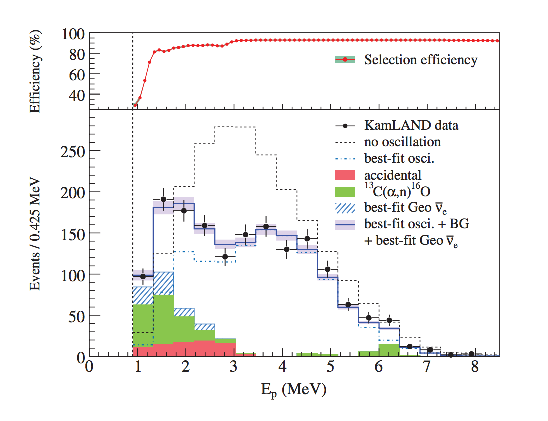
\includegraphics[width=0.75\textwidth]{kamland_reactor_spectrum}
  \caption[Kamland Reactor Spectrum]{Reactor anti-neutrino energy spectrum observed by KamLAND.
                                    Figure from~\cite{kamland_reactor}.}
  \label{fig:kamland_reactor}
\end{figure}

Figure~\ref{fig:kamland_reactor} shows reactor anti-neutrino energy spectrum measured
by the KamLAND experiment, with the best fit mixing parameters compared to the
expected spectrum with no oscillations.
From this measurement a best fit value of $\Delta m^{2}_{21} = 7.58^{+0.14}_{-0.13}(\mathrm{stat.})^{+0.15}_{-0.15}(\mathrm{syst.}) \times 10^{-5}$\,eV
and $\tan^{2} \theta_{12} = 0.56^{+0.10}_{-0.07}(\mathrm{stat.})^{+0.10}_{-0.06}(\mathrm{syst.})$ was determined.

The value for $\Delta m^{2}_{21}$ measured by KamLAND is in disagreement with the value extracted
by solar experiments, although it cannot be ruled out that the disagreement
is a result of a statistical fluctuation. This discrepancy will be discussed further
in section~\ref{sec:chameleons}.

